%==============================================
\begin{frame}{Overview}
%==============================================
\begin{itemize}
  \item Seismic data acquisition
   \item CMP method
   \item NMO and stack
   \item Velocity analysis
  \end{itemize}
\end{frame}
%-------------------------------------------------
\begin{frame}{Seismic marine data acquisition}
%-------------------------------------------------
%
\begin{figure}
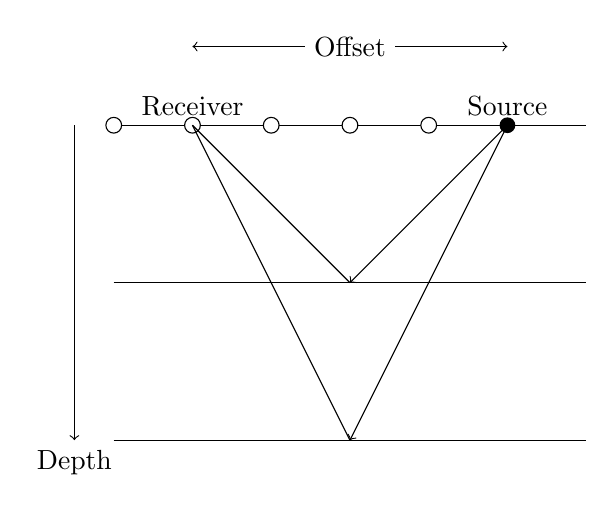
\begin{tikzpicture}
  \draw[->] (-0.5,4.0) -- (-0.5,0.0) node[below]{Depth} ;
  \draw[<->] (1.0,5.0) -- node[fill=white]{Offset} (5.0,5.0); 
  \draw (0.0,0.0) -- (6.0,0.0) ;
  \draw (0.0,2.0) -- (6.0,2.0) ;
  \draw (0.0,4.0) -- (6.0,4.0) ;
  \fill (5.0,4.0) node[above]{Source} circle (0.1) ;
  \fill[white] (0.0,4.0) circle (0.1) ;
  \draw (0.0,4.0) circle (0.1) ;
  \fill[white](1.0,4.0) circle (0.1) ;
  \draw (1.0,4.0) node[above]{Receiver}circle (0.1) ;
  \fill[white] (2.0,4.0) circle (0.1) ;
  \draw (2.0,4.0) circle (0.1) ;
  \fill[white] (3.0,4.0) circle (0.1) ;
  \draw (3.0,4.0) circle (0.1) ;
  \fill[white] (4.0,4.0) circle (0.1) ;
  \draw (4.0,4.0) circle (0.1) ;
  \draw[->] (5.0,4.0) -- (3.0,0.0) ;
  \draw (3.0,0.0) -- (1.0,4.0) ;
  \draw[->] (5.0,4.0) -- (3.0,2.0) ;
  \draw (3.0,2.0) -- (1.0,4.0) ;
\end{tikzpicture}
\label{fig:geom}
\end{figure}
\end{frame}
%
%-----------------------------------------
\begin{frame}{Schematic shot record}
%-----------------------------------------
%
\plot{schemshot}{width=0.5\textwidth}{}
%
\end{frame}
%----------------------------------------------
\begin{frame}{Real shot record}
%----------------------------------------------
%
\plot{shotgath}{width=0.5\textwidth}{}
%
\end{frame}
%-----------------------------------------
\begin{frame}{The cmp method}
%-----------------------------------------
%
\begin{figure}
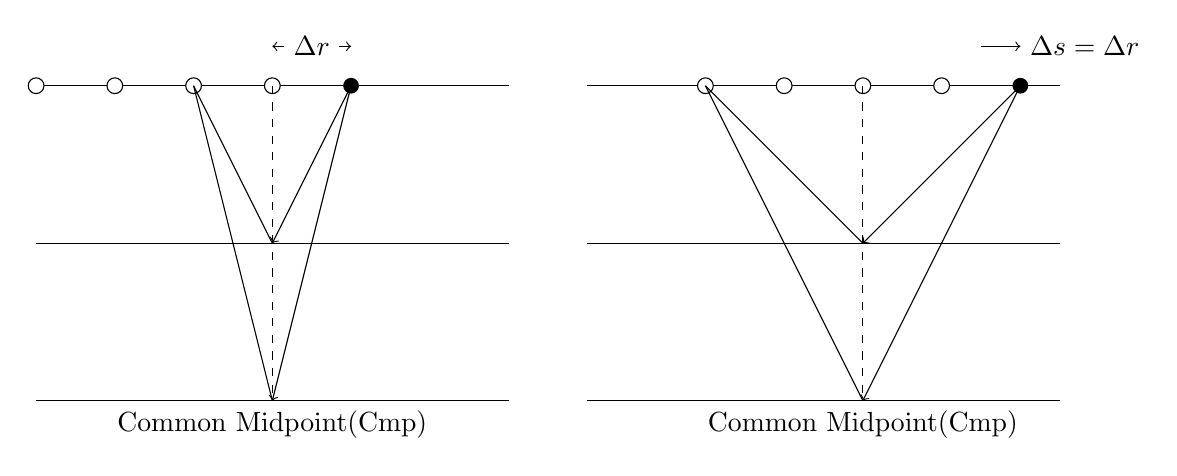
\begin{tikzpicture}
  \draw[<->] (3.0,4.5) -- node[fill=white]{$\Delta r$}(4.0,4.5); % Draw Delta r 
  \draw (0.0,0.0) -- (6.0,0.0) ;     %Draw Bottom reflector left display
  \draw (0.0,2.0) -- (6.0,2.0) ;     %Draw Middle reflector left display
  \draw (0.0,4.0) -- (6.0,4.0) ;     %Draw Surface left display
  \fill (4.0,4.0) circle (0.1) ;     %Draw source left display

  %Draw receivers on left display 

  \fill[white] (0.0,4.0) circle (0.1) ; 
  \draw (0.0,4.0) circle (0.1) ;
  \fill[white] (1.0,4.0) circle (0.1) ;
  \draw (1.0,4.0) circle (0.1) ;
  \fill[white] (2.0,4.0) circle (0.1) ;
  \draw (2.0,4.0) circle (0.1) ;
  \fill[white] (3.0,4.0) circle (0.1) ;
  \draw (3.0,4.0) circle (0.1) ;
 
  % Draw dashed vertical line and cmp text below bottom reflector left display
  \draw[dashed] (3.0,4.0) -- (3.0,0.0) node[below]{Common Midpoint(Cmp)} ;

  %Draw raypaths to bottom layer left display
  \draw[->] (4.0,4.0) -- (3.0,0.0) ; 
  \draw (3.0,0.0) -- (2.0,4.0) ;     

  %Draw raypaths to middle layer left display
  \draw[->] (4.0,4.0) -- (3.0,2.0) ;
  \draw (3.0,2.0) -- (2.0,4.0) ;

  \draw (7.0,0.0) -- (13.0,0.0) ; Draw bottom reflector right display
  \draw (7.0,2.0) -- (13.0,2.0) ; Draw middle reflector right display
  \draw (7.0,4.0) -- (13.0,4.0) ; Draw surface right display

  % Draw Delta s headline
  \fill (12.5,4.0) circle (0.1) ;
  \draw[->] (12.0,4.5) -- (12.5,4.5) node[right]{$\Delta s=\Delta r$};

  %Draw receivers on right display 
  \fill[white] (8.5,4.0)  circle (0.1) ;
  \draw (8.5,4.0)  circle (0.1) ;
  \fill[white] (9.5,4.0)  circle (0.1) ;
  \draw (9.5,4.0)  circle (0.1) ;
  \fill[white] (10.5,4.0) circle (0.1) ;
  \draw (10.5,4.0) circle (0.1) ;
  \fill[white] (11.5,4.0) circle (0.1) ;
  \draw (11.5,4.0) circle (0.1) ;

  %Draw raypaths to bottom layer
  \draw[->] (12.5,4.0) -- (10.5,0.0) ;
  \draw (10.5,0.0) -- (8.5,4.0) ;

  %Draw raypaths to middle layer
  \draw[->] (12.5,4.0) -- (10.5,2.0) ;
  \draw (10.5,2.0) -- (8.5,4.0) ;

  % Draw dashed vertical line and cmp text below bottom reflector left display
  \draw[dashed] (10.5,4.0) -- (10.5,0.0)node[below]{Common Midpoint(Cmp)} ;

\end{tikzpicture}
\label{fig:shotsgeom}
\end{figure}
%
\end{frame}
%--------------------------------------------
\begin{frame}{Common midpoint (cmp) gather}
%--------------------------------------------
\begin{figure}
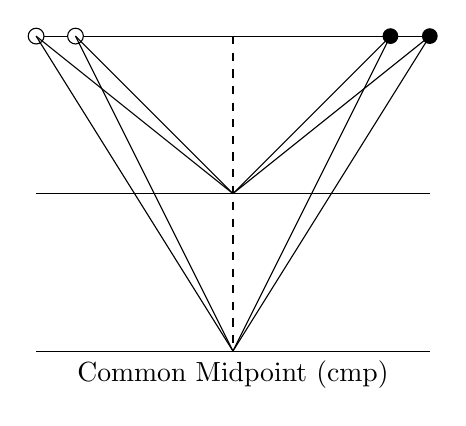
\begin{tikzpicture}
  \draw (0.0,0.0) -- (5.0,0.0) ;
  \draw (0.0,2.0) -- (5.0,2.0) ;
  \draw (0.0,4.0) -- (5.0,4.0) ;
  \fill[white] (0.0,4.0) circle (0.1) ;
  \draw (0.0,4.0) circle (0.1) ;
  \fill (5.0,4.0) circle (0.1) ;
  \fill[white] (0.5,4.0) circle (0.1) ;
  \draw (0.5,4.0) circle (0.1) ;
  \fill (4.5,4.0) circle (0.1) ;
  \draw[dashed] (2.5,4.0) -- (2.5,0.0)node[below]{Common Midpoint (cmp)} ;
  \draw (5.0,4.0) -- (2.5,2.0) ;
  \draw (2.5,2.0) -- (0.0,4.0) ;
  \draw (4.5,4.0) -- (2.5,2.0) ;
  \draw (2.5,2.0) -- (0.5,4.0) ;

  \draw (5.0,4.0) -- (2.5,0.0) ;
  \draw (2.5,0.0) -- (0.0,4.0) ;
  \draw (4.5,4.0) -- (2.5,0.0) ;
  \draw (2.5,0.0) -- (0.5,4.0) ;
\end{tikzpicture}
\label{fig:1-cmp}
\end{figure}
\end{frame}
%
%--------------------------------------------
\begin{frame}{Midpoint and Offset Coordinates}
%--------------------------------------------
\begin{eqnarray}
x_m & = & \frac{s+r}{2} ,\\
h   & = &  \frac{s-r}{2},
\label{eq:cmpcoord}
\end{eqnarray}
\begin{itemize}
  \item $x_m$: Midpoint coordinate
  \item $h$: Offset
  \item $s$: Source coordinate
  \item $r$: Receiver coordinate
\end{itemize}
\end{frame}
%-----------------------------------------
\begin{frame}{NMO and Stack}
%-----------------------------------------
\begin{figure}
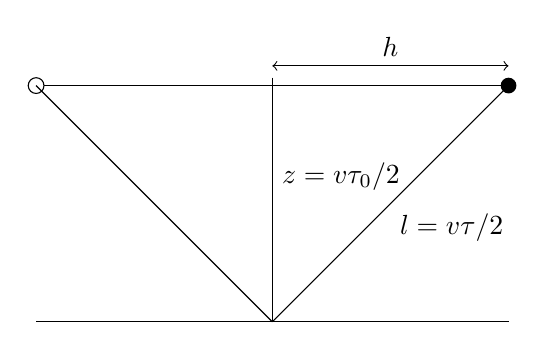
\begin{tikzpicture}
  \draw (0.0,1.0) -- (6.0,1.0) ;
  \draw (0.0,4.0) -- (6.0,4.0) ;
  \draw[<->](3.0,4.25) -- node[above]{$h$}(6.0,4.25) ;
  \fill[white] (0.0,4.0) circle (0.1) ;
  \draw (0.0,4.0) circle (0.1) ;
  \fill (6.0,4.0) circle (0.1) ;
  \draw (6.0,4.0) -- node[below right]{$l=v\tau/2$}(3.0,1.0) ;
  \draw (3.0,1.0) -- (0.0,4.0) ;
  \draw (3.0,4.1) -- node[above right]{$z=v\tau_0/2$}(3.0,1.0) ;
\end{tikzpicture}
\label{fig:nmop}
\end{figure}

The traveltime $\tau(h)$ is:
%
\begin{eqnarray}
l^2 = z^2+h^2 \nonumber\\
\end{eqnarray}
which gives by inserting $v\tau/2$ for $l$ and $v\tau_0/2$ for $z$
\begin{eqnarray}
\tau(h)=\sqrt{t^2_0+4h^2/v^2}.
\label{eq:nmo}
\end{eqnarray}
\end{frame}
%-----------------------------------------
\begin{frame}{NMO and Stack}
%-----------------------------------------
Nmo-correction:
%
\begin{eqnarray}
 \Delta \tau = \tau(h)-\tau_0,
\label{eq:dtnmo}
\end{eqnarray}
\end{frame}
%
%-----------------------------------------
\begin{frame}{Cmp}
%-----------------------------------------
 \plot{synshot}{width=0.50\textwidth}{} 
\end{frame}
%-----------------------------------------
\begin{frame}{Nmo}
%-----------------------------------------
 \plot{syncmp}{width=0.50\textwidth}{} 
\end{frame}
%-----------------------------------------
\begin{frame}{Stack}
%-----------------------------------------
 \plot{synstack}{width=0.50\textwidth}{} 
\end{frame}
%-----------------------------------------
\begin{frame}{NMO and Stack}
%-----------------------------------------
Average velocity $v_{rms}$ defined by
\begin{eqnarray}
 v^2_{rms}(t_0)=\frac{1}{t_0}\int^{t_0}_0 v^2(t)dt
\label{eq:rms}
\end{eqnarray}
$v(t)$ : Interval velocity.
The traveltime equation \eqref{eq:nmo} then becomes
\begin{eqnarray}
\tau(h)=\sqrt{t^2_0+4h^2/v^2_{rms}(t_0)}.
\label{eq:nmorms}
\end{eqnarray}
\end{frame}
%-----------------------------------------
\begin{frame}{Velocity analysis}
%-----------------------------------------
%
  Estimate $v_{rms}$ from equation \eqref{eq:nmo}
\begin{enumerate}
  \item Make a guess of $v$ 
  \item Perform Nmo correction for all $t_0$ with using guess of $v$
  \item Make a stack trace
  \item Perform above steps for a range of guesses of $v$
  \item Plot all stack traces in a velocity spectrum
\end{enumerate}
\end{frame}
%-----------------------------------------
\begin{frame}{Velocity spectrum}
%-----------------------------------------
 \plot{synscn}{width=0.5\textwidth}{}
\end{frame}
%-----------------------------------------
\begin{frame}{Semblance}
%-----------------------------------------
Stack is usually replaced with semblance to
get better velocity spectra  
\begin{eqnarray}
S(t) = \frac{\int_0^{h_{max}} p^2(t,h)}{\int dt_0^T\, \int_0^{h_{max}} p^2(t,h)}
\end{eqnarray}
\begin{itemize}
 \item $p(t,h)$ : data 
 \item $h_{max}$: maximum offset. 
\end{itemize}
This equation can not be used directly.  Why?
\end{frame}
%
%-----------------------------------------
\begin{frame}{Semblance}
%-----------------------------------------
\begin{eqnarray}
S_k = \frac{\sum_{i=0}^{N_h} p^2_{k,i}}{\sum_{k=0}^{N_t} \sum_{i=0}^{N_h} p^2_{k,i}}
\end{eqnarray}
\begin{itemize}
 \item $S_k = S(t=k\Delta t), k=0,\ldots,N_t$ 
 \item $p_{k,i}=p(t=k\Delta t,h=i\Delta h), i=0,\ldots,N_h$. 
 \item $\Delta t$ time sampling interval, 
 \item $\Delta h$ distance between offsets \item $N_t$,$N_h$ :
No of time samples and No of  offsets
\end{itemize}
\end{frame}
%-----------------------------------------
\begin{frame}{Velocity analysis}
%-----------------------------------------
 \plot{synvel}{width=0.5\textwidth}{}
\end{frame}
%-----------------------------------------
\begin{frame}{Velocity analysis}
%-----------------------------------------
 \plot{cmp}{width=0.5\textwidth}{}
\end{frame}
%-----------------------------------------
\begin{frame}{Velocity analysis}
%-----------------------------------------
 \plot{scn-1}{width=0.5\textwidth}{}
\end{frame}
%-----------------------------------------
\begin{frame}{Velocity analysis}
%-----------------------------------------
 \plot{nmo}{width=0.5\textwidth}{}
\end{frame}
%-----------------------------------------
\begin{frame}{Velocity analysis}
%-----------------------------------------
 \plot{stack}{width=0.75\textwidth}{}
\end{frame}
%--------------------------------------------
\begin{frame}{Summary}
%--------------------------------------------
\begin{itemize}
  \item Seismic data acquisition
   \item CMP method
   \item NMO-correction
   \item Velocity analysis
  \end{itemize}
%
\end{frame}
